\section{Results and Discussion}\label{sec:results}

\subsection{Setup}\label{sec:setup}
Every number and curve in this section is computed with \cref{alg:force}. The scripts \texttt{code/make\_results.py},
\texttt{code/make\_results2.py} and \texttt{figures/make\_figures.py} regenerate them. Unless stated otherwise,
$\varepsilon=1$, $\mu_s=\mu_p=\mu$, $\beta_s=0$ and $\hat\ell_c=0$ (\cref{tab:params}). The rigid no-slip sphere near a
rigid no-slip wall, the configuration of Zhang \emph{et al.}~\cite{zhang2023unsteady}, is the baseline: it is the limit
$\gamma=1$, $\alpha_p\to\infty$ of the present model, so every difference from it isolates the effect of
permeability. The steady limit is the second baseline: it isolates the effect of fluid inertia at fixed geometry and
corresponds to the setting of Ref.~\onlinecite{faltas2021axisymmetric}. Following \cref{rem:accuracy}, quantitative
statements are restricted to $\varepsilon\ge1$.

\begin{table}[t]
\caption{Parameters of the computations.}
\label{tab:params}
\begin{ruledtabular}
\begin{tabular}{lll}
Quantity & Values & Used in\\
\hline
$\Wo$ & $0.05$--$50$ (46 log-spaced) & \cref{fig:spectra,fig:soft}\\
$\varepsilon$ & $0.25$--$5$ & \cref{fig:validation,fig:steady,fig:acoustic}\\
$\alpha_p$ & $3$--$100$ (11 log-spaced); $5,10,20,50,\infty$ & \cref{fig:woc_ap,fig:spectra}\\
$\beta_p$ & $-0.5,\ 0,\ 0.5$ & \cref{fig:woc_ap,fig:steady}\\
$\gamma$ & $0,\ 0.5,\ 0.7,\ 0.8,\ 0.95,\ 1$ & \cref{fig:soft}\\
$\alpha_s$ & $1$--$50$ & \cref{fig:soft}\\
CTC-like particle & $\gamma=0.9$, $\alpha_s=20$ & \cref{fig:acoustic}\\
leukocyte-like particle & $\gamma=0.7$, $\alpha_s=5$ & \cref{fig:acoustic}\\
\end{tabular}
\end{ruledtabular}
\end{table}

\subsection{Validation}\label{sec:validation}

\begin{table}[t]
\caption{Validation. Top: unbounded fluid; $\hat F_\infty$ for the rigid sphere at $\Wo=2$ and the porous-sphere drag
ratio $\Omega=\hat F_\infty/(-6\pi)$ at $\Wo=10^{-4}$ against the Debye--Bueche--Brinkman (DBB) formula. Bottom: steady
($\Wo\to0$) wall correction $F/F_\infty$ for a rigid sphere near a rigid wall.}
\label{tab:validation}
\begin{ruledtabular}
\begin{tabular}{lcc}
Case & Present & Reference\\
\hline
Rigid, $\Wo=2$: $\hat F_\infty$ & $-45.5069+35.0349i$ & $-45.5069+35.0349i$ [Eq.~\eqref{eq:rigid_BC}]\\
Porous, $\alpha_s=1$: $\Omega$ & $0.17561$ & $0.17561$ (DBB)\\
Porous, $\alpha_s=5$: $\Omega$ & $0.76342$ & $0.76338$ (DBB)\\
Porous, $\alpha_s=20$: $\Omega$ & $0.94669$ & $0.94663$ (DBB)\\
\hline
 & normal: present / Brenner~\cite{brenner1961slow} & parallel: present / Faxén series\\
$\varepsilon=0.5$ & $2.639$ / $3.205$ & $1.530$ / $1.615$\\
$\varepsilon=1$ & $2.018$ / $2.126$ & $1.365$ / $1.386$\\
$\varepsilon=2$ & $1.555$ / $1.569$ & $1.224$ / $1.227$\\
$\varepsilon=3$ & $1.377$ / $1.380$ & $1.161$ / $1.162$\\
$\varepsilon=4$ & $1.284$ / $1.285$ & $1.125$ / $1.126$\\
\end{tabular}
\end{ruledtabular}
\end{table}

\begin{figure*}[t]
  \centering
  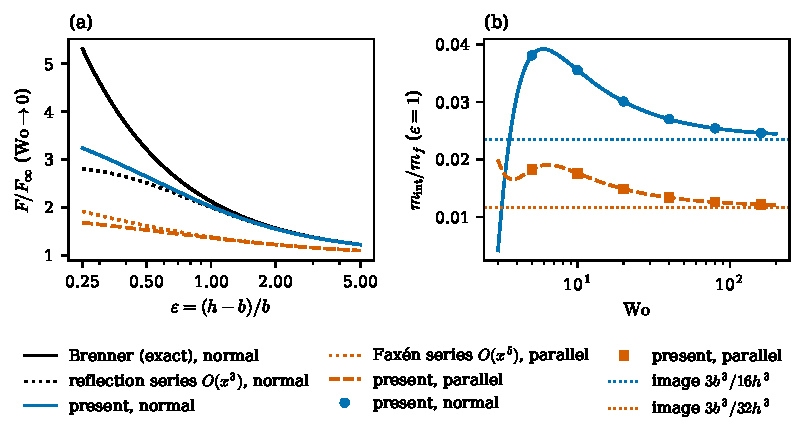
\includegraphics[width=0.85\textwidth]{figures/fig2_validation.pdf}
  \caption{Validation for a rigid sphere near a rigid wall. (a) Steady wall correction against Brenner's exact
  solution~\cite{brenner1961slow} and the classical reflection series (normal), and against Faxén's series (parallel).
  (b) Wall-induced added mass at $\varepsilon=1$ against the inviscid image values of \cref{prop:inviscid}.}
  \label{fig:validation}
\end{figure*}

\Cref{tab:validation} shows that the sphere solver reproduces the exact unsteady drag of a rigid sphere to all
printed digits. It also reproduces the Debye--Bueche--Brinkman drag of a porous sphere; the residual difference of
$<10^{-4}$ is the $O(\Wo)$ unsteady correction at $\Wo=10^{-4}$. \Cref{fig:validation}(a) compares the steady wall
correction with Brenner's exact series~\cite{brenner1961slow}. The dipolar closure follows the classical reflection
series through $O(x^3)$, as expected from \cref{rem:accuracy}. Its error relative to the exact solution is $5.1\%$ at
$\varepsilon=1$, $0.9\%$ at $\varepsilon=2$ and $<0.3\%$ for $\varepsilon\ge3$ in normal motion. Parallel motion is more accurate: it differs by $1.5\%$ from Faxén's fifth-order series at $\varepsilon=1$, because
the leading neglected coefficient is smaller. At $\varepsilon=0.5$
the error grows to $18\%$ (normal), confirming that the lubrication regime needs higher multipoles.
\Cref{fig:validation}(b) shows the high-frequency check. The wall-induced added mass decreases monotonically towards
the image values $3/(16h^3)=0.0234$ (normal) and $3/(32h^3)=0.0117$ (parallel) of \cref{prop:inviscid}: at $\Wo=160$ the
present values are $0.0246$ and $0.0122$. The remaining $5\%$ comes from higher image reflections, which the closure
retains, and from the $O(\Wo^{-1})$ boundary layers. The model therefore captures both ends of the frequency range.

\subsection{Rigid sphere: from a rigid wall to a permeable layer}\label{sec:rigid_results}

\begin{figure*}[t]
  \centering
  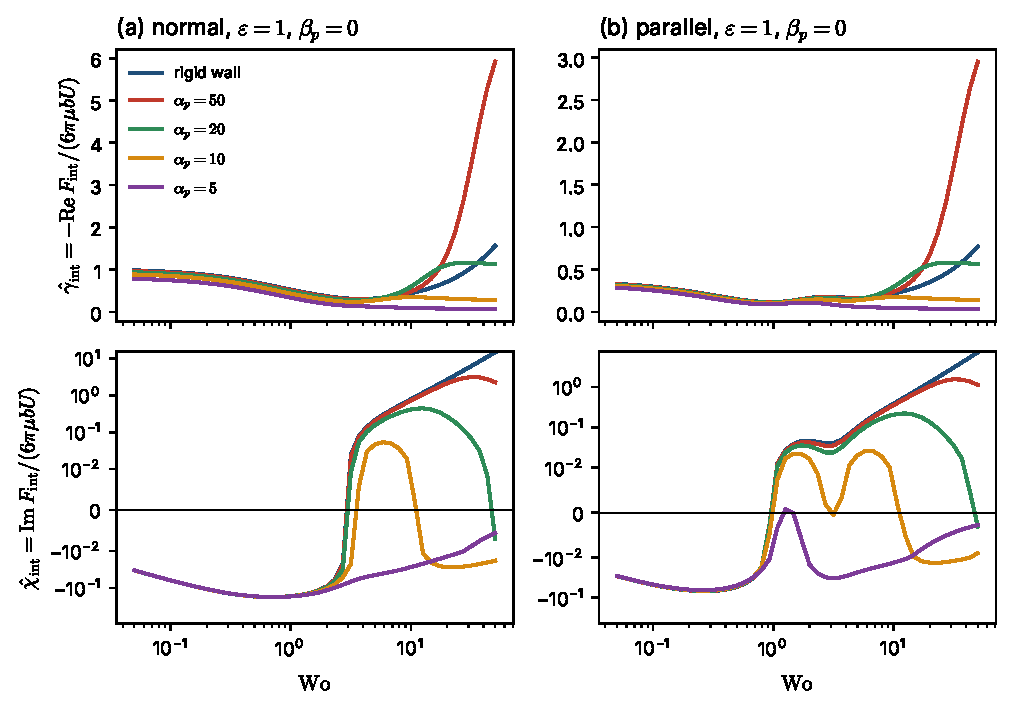
\includegraphics[width=0.85\textwidth]{figures/fig3_spectra_alphap.pdf}
  \caption{Interaction spectra of a rigid sphere at $\varepsilon=1$, $\beta_p=0$, for a rigid wall and layers with
  $\alpha_p=50,20,10,5$. Top: wall-induced damping $\hat\gamma_{\rm int}$. Bottom: reactive coefficient
  $\hat\chi_{\rm int}=\omega m_{\rm int}/(6\pi\mu b)$ (symmetric-log axis); its sign is that of $m_{\rm int}$. (a) Normal,
  (b) parallel oscillation.}
  \label{fig:spectra}
\end{figure*}

\Cref{fig:spectra} shows the wall-induced damping and reactive force as functions of $\Wo$. Near a rigid wall (blue)
the damping falls from its steady value $\hat\gamma_{\rm int}=0.98$ (normal) to a minimum of $0.31$ at $\Wo\approx3.7$,
then rises again, because the Stokes layer that forms on the wall dissipates more energy as $\Wo$ grows. The reactive
part is negative for $\Wo<\Wo_c=2.92$ and positive above it (normal); for parallel oscillation the crossover is at
$\Wo_c=0.955$. The negative branch has a simple interpretation. In unbounded fluid the Basset memory term
$-6\pi\lambda$ contributes a positive reactive force $6\pi\Wo/\sqrt2$, carried by vorticity that diffuses to distances
$|\lambda_f|^{-1}\gg h$ when $\Wo\ll1$. The wall truncates this diffusion, so it removes part of the memory force,
which appears as a negative added mass. Once $|\lambda_f|^{-1}\lesssim h$ the vorticity no longer reaches the wall,
and the reactive interaction is dominated by the potential image of \cref{prop:inviscid}, which is positive. With
\cref{rem:sign}, this reproduces the change of sign of the AFM resonance-frequency shift reported by Zhang
\emph{et al.}~\cite{zhang2023unsteady}.

A permeable layer changes this picture in three ways. First, in the steady limit the layer lets fluid escape through
the interface, so the damping is smaller: $\hat\gamma_{\rm int}(\Wo\to0)=0.94$, $0.89$ and $0.78$ for $\alpha_p=20$, $10$
and $5$ (normal). Second, at high frequency the reactive force does not keep growing. It peaks and then changes sign a
second time, because the layer becomes transparent to the oscillatory disturbance (\cref{rem:transparent}). Third, for
$\alpha_p=5$ the reactive force stays negative at all frequencies: the window of positive added mass has disappeared.
At $\Wo\approx\alpha_p$ the damping also shows a pronounced maximum, e.g.\ $\hat\gamma_{\rm int}=5.9$ at $\Wo=50$ for
$\alpha_p=50$, which is four times the rigid-wall value. This is the frequency at which the Stokes-layer thickness
matches the Brinkman screening length, so the oscillatory flow penetrates the layer and does work against its Darcy
drag. A rigid wall has no such dissipation channel.

\subsection{Crossover map: a frequency fingerprint of layer permeability}\label{sec:woc_results}

\begin{figure*}[t]
  \centering
  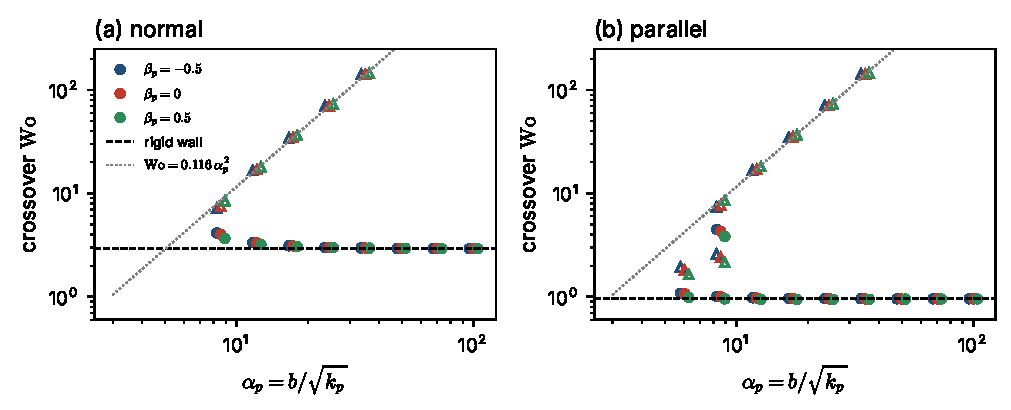
\includegraphics[width=0.85\textwidth]{figures/fig4_Woc_alphap.pdf}
  \caption{All crossover Womersley numbers of $m_{\rm int}$ against layer permeability at $\varepsilon=1$, for
  $\beta_p=-0.5,0,0.5$ (markers slightly offset horizontally). Filled circles: upward crossovers $\Wo_c^{\uparrow}$;
  open triangles: downward crossovers $\Wo_c^{\downarrow}$. Dashed: rigid-wall value. Dotted: fit
  $\Wo_c^{\downarrow}=0.116\,\alpha_p^2$. Upper crossovers above the scanned range ($\Wo\le\max(150,2.5\alpha_p)$) are not
  shown. (a) Normal, (b) parallel oscillation.}
  \label{fig:woc_ap}
\end{figure*}

\Cref{fig:woc_ap} collects all crossovers. Three features stand out.

\emph{(i) The lower crossover rises as the layer becomes more permeable.} For normal oscillation with $\beta_p=0$,
$\Wo_c^{\uparrow}=2.92$ (rigid wall), $2.96$ ($\alpha_p=35$), $3.10$ ($\alpha_p=17$) and $4.01$ ($\alpha_p=8.6$). The
shift is monotonic and becomes steep as $\alpha_p$ approaches about $10$, which is where the method is most sensitive.

\emph{(ii) An upper crossover scales as $\alpha_p^2$.} The downward crossover follows
$\Wo_c^{\downarrow}\approx0.116\,\alpha_p^2$ at $\varepsilon=1$: a least-squares fit gives exponent $2.08$, and
$\Wo_c^{\downarrow}/\alpha_p^2$ lies within $0.112$--$0.116$ for $\alpha_p\ge12$. The scaling is quadratic, not the naive $\Wo\sim\alpha_p$
suggested by \cref{eq:lambdas_nd}. In dimensional form it states that the viscous penetration depth at the upper
crossover is $\sqrt{\mu/\rho\omega}\approx8.6\,k_p/b$: the layer becomes transparent once the oscillatory boundary
layer is thinner than a length that combines the pore scale $\sqrt{k_p}$ with the ratio $\sqrt{k_p}/b$. For a probe of
known size, the upper crossover therefore measures $k_p$ directly. \TODO{authors: consider an asymptotic derivation of the prefactor $0.116$
and of its $\varepsilon$ dependence.}

\emph{(iii) The positive-added-mass window closes.} Below a threshold permeability no crossover exists in the scanned range, and the wall-induced added mass is negative
at all frequencies. The window closes between $\alpha_p=6.1$ and $8.6$ for normal oscillation, and between $4.3$ and
$6.1$ for parallel oscillation. For parallel oscillation near the threshold ($\alpha_p=8.6$) the window splits into two,
with four crossovers.

The stress jump $\beta_p$ has a weaker, systematic effect. A positive $\beta_p$, which increases the tangential momentum
transfer into the layer, lowers $\Wo_c^{\uparrow}$ (e.g.\ $3.64$ vs.\ $4.14$ for $\beta_p=0.5$ and $-0.5$ at
$\alpha_p=8.6$) and raises $\Wo_c^{\downarrow}$ slightly, so it widens the window. Its influence fades for
$\alpha_p\gtrsim30$.

\emph{Implication for microrheology.} A frequency sweep of the near-wall force of a colloidal probe at fixed $\varepsilon$
measures up to two crossovers. Each is a monotonic function of $\alpha_p$ in a different range: $\Wo_c^{\uparrow}$ is
sensitive for $\alpha_p\lesssim30$, and $\Wo_c^{\downarrow}$ for larger $\alpha_p$. Together they provide a non-contact
estimate of the layer permeability, for example to monitor degradation of the glycocalyx, which increases $k_p$.
\TODO{authors: map to dimensional AFM frequencies for a $b=5$--$20\,\mu$m probe in water and $k_p$ values from the
glycocalyx literature.}

\subsection{Steady limit}\label{sec:steady_results}
\begin{figure}[t]
  \centering
  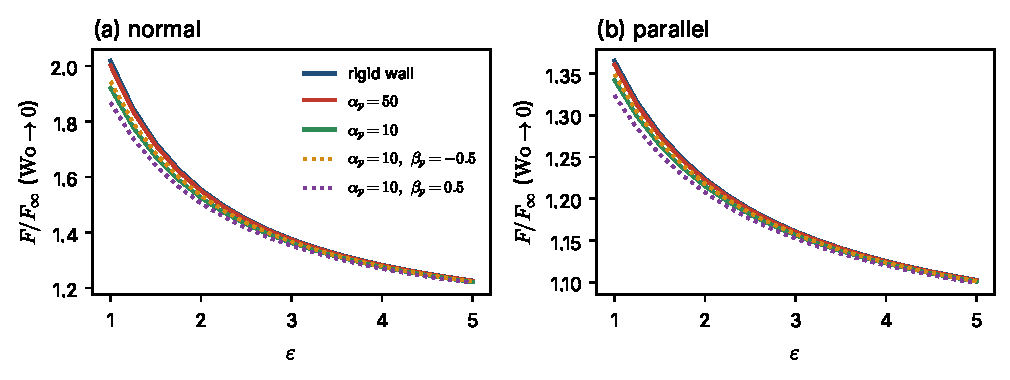
\includegraphics[width=\linewidth]{figures/fig6_steady.pdf}
  \caption{Steady ($\Wo\to0$) resistance of a rigid sphere against gap, for a rigid wall and for layers with
  $\alpha_p=50$ and $10$ and stress jumps $\beta_p=\pm0.5$. (a) Normal, (b) parallel.}
  \label{fig:steady}
\end{figure}
\Cref{fig:steady} shows the zero-frequency limit, where our formulation reduces to the problem of
Ref.~\onlinecite{faltas2021axisymmetric} (for normal motion) and extends it to parallel motion. Permeability lowers the
resistance, at $\varepsilon=1$ from $2.018$ (rigid wall) to $1.921$ ($\alpha_p=10$, normal) and from $1.365$ to $1.342$
(parallel). A positive $\beta_p$ lowers the resistance further ($1.867$ for
$\beta_p=0.5$) and a negative one raises it ($1.943$). All curves merge for $\varepsilon\gtrsim4$. Compared with the
unsteady crossovers, which shift by tens of per cent, the steady drag changes by only a few per cent. A frequency
sweep is therefore a far more sensitive probe of the layer than a steady drag measurement.

\subsection{Soft particles}\label{sec:soft_results}
\begin{figure*}[t]
  \centering
  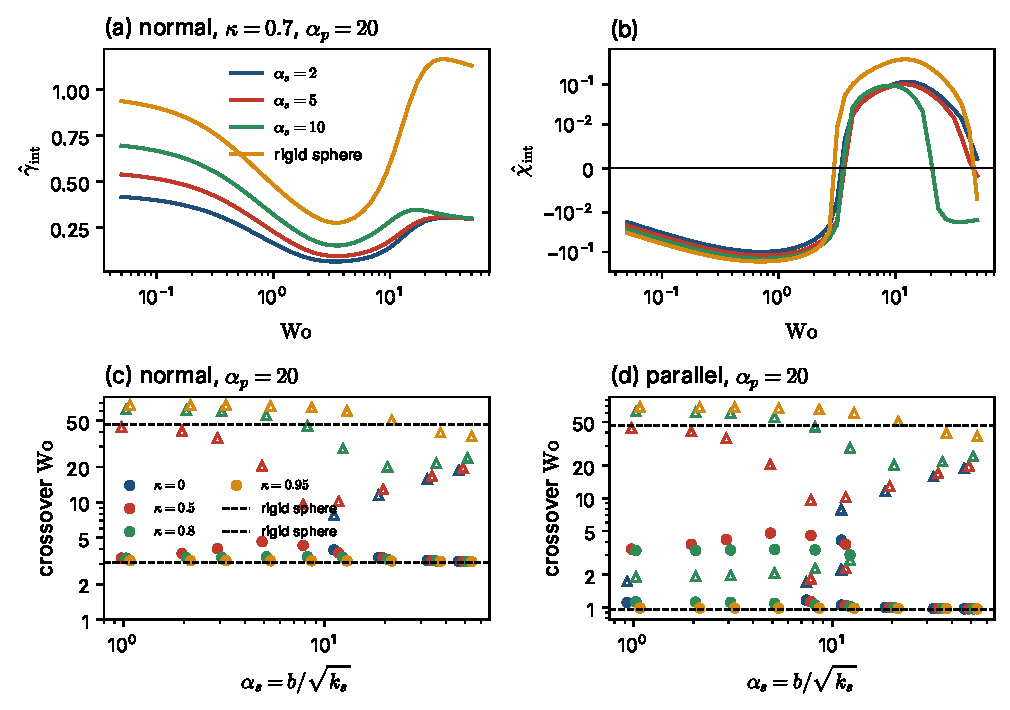
\includegraphics[width=0.85\textwidth]{figures/fig5_soft_particle.pdf}
  \caption{Soft core--shell particles near a glycocalyx-like layer ($\alpha_p=20$, $\beta_p=0$, $\varepsilon=1$).
  (a,b) Spectra for $\gamma=0.7$ and $\alpha_s=2,5,10$ against a rigid sphere (normal). (c,d) All crossover Womersley
  numbers against shell permeability for $\gamma=0,0.5,0.8,0.95$ (circles: upward; triangles: downward); dashed: rigid
  sphere.}
  \label{fig:soft}
\end{figure*}

\Cref{fig:soft}(a) shows that a permeable shell substantially reduces the wall-induced damping. For $\gamma=0.7$ the
steady value falls from $0.94$ (rigid) to $0.70$, $0.54$ and $0.42$ for $\alpha_s=10$, $5$ and $2$, and the minimum near
$\Wo\approx3.5$ falls from $0.28$ to $0.07$. Fluid passes through the shell instead of being squeezed out of the gap.
The high-frequency damping peak caused by the layer persists, but it is weaker because the scattered field is weaker.
The reactive part [\cref{fig:soft}(b)] keeps its crossover at $\Wo\approx3$--$4$, while its positive maximum is
reduced by a factor of about four.

The crossover maps [\cref{fig:soft}(c,d)] show a strong dependence on particle structure:
\begin{itemize}
\item \emph{Thin shells} ($\gamma=0.95$) behave like rigid spheres: $\Wo_c^{\uparrow}\approx3.18$ (normal) and $0.99$
      (parallel), independent of $\alpha_s$.
\item \emph{Homogeneous porous particles} ($\gamma=0$) lose the crossover in normal oscillation for $\alpha_s\le8$, so
      their wall-induced added mass is negative at all frequencies. For larger $\alpha_s$ the window reappears, with
      $\Wo_c^{\uparrow}=3.94$ at $\alpha_s=12$, decreasing towards the rigid value.
\item \emph{Intermediate cores} ($\gamma=0.5$) show a non-monotonic $\Wo_c^{\uparrow}(\alpha_s)$ with a maximum of $4.6$
      at $\alpha_s=5$ (normal). In parallel oscillation the low crossover near $\Wo\approx1$ disappears for
      $\alpha_s\le5$, and the first crossover jumps to $\Wo=3.4$--$4.8$. For $\gamma=0.8$ and $\alpha_s\le12$, parallel
      oscillation has two separate positive windows (four crossovers).
\end{itemize}
The upper crossover $\Wo_c^{\downarrow}$ also depends on the particle. It falls from $46$ (rigid sphere) to
$8$--$20$ for homogeneous porous particles and for $\gamma=0.5$ with $\alpha_s\ge8$. A weaker scattered field is
cancelled earlier by the transparency of the layer. \TODO{authors: confirm this interpretation.}

\emph{Implication for carriers.} A permeable shell lowers the near-wall damping by up to a factor of four and removes
the positive-added-mass window. Such a particle therefore experiences less resistance when driven near a mucus layer,
which supports the use of soft, PEG-like shells in mucus-penetrating carriers~\cite{pangeni2023airway}. The core slip
$\hat\ell_c$ is included in the model but has a weaker effect when the shell is permeable. \TODO{authors: add a panel
or table varying $\hat\ell_c$ and $\beta_s$ if the reviewers ask.}

\subsection{Acoustofluidic contrast between cell-like particles}\label{sec:acoustic_results}
\begin{figure*}[t]
  \centering
  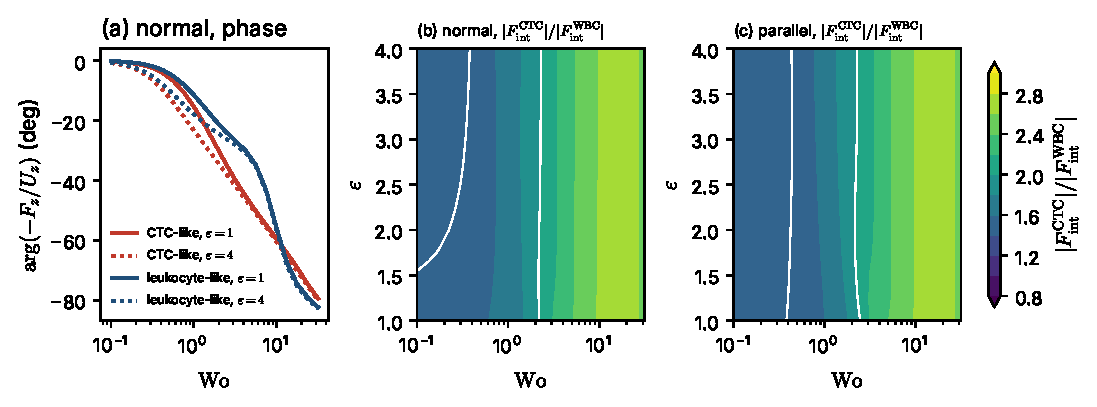
\includegraphics[width=0.9\textwidth]{figures/fig7_acoustic_contrast.pdf}
  \caption{CTC-like ($\gamma=0.9$, $\alpha_s=20$) against leukocyte-like ($\gamma=0.7$, $\alpha_s=5$) particles of equal outer
  radius near an endothelial-like layer ($\alpha_p=20$, $\beta_p=0$). (a) Phase of the total resistance at
  $\varepsilon=1$ and $4$ (normal). (b,c) Ratio of the magnitudes of the wall-induced forces (white contours: $1$, $1.5$,
  $2$).}
  \label{fig:acoustic}
\end{figure*}

As an illustration for acoustofluidic sorting~\cite{wu2019acoustofluidic,hossein2023review}, \cref{fig:acoustic}
compares two particles of the same outer radius, a stiffer CTC-like particle and a softer leukocyte-like particle. The
parameters in \cref{tab:params} are representative, not fitted to specific cell lines. The phase of the total resistance
[\cref{fig:acoustic}(a)] differs by up to $13^\circ$ near $\Wo\approx3$ and by less than $1^\circ$ for $\Wo\lesssim0.3$. The
wall-induced force of the CTC-like particle is $1.4$--$2.7$ times larger [\cref{fig:acoustic}(b,c)]. The ratio depends
mainly on $\Wo$ and only weakly on $\varepsilon$, and it is largest for $\Wo\gtrsim5$. The wall-induced force is a
significant fraction of the total only close to the layer: at $\varepsilon=1$, $|F_{\rm int}|/|F_\infty|=0.78$ (normal)
at $\Wo=0.1$, but $0.04$ at $\Wo=10$. Near-wall sorting by softness therefore works best at moderate frequencies,
$\Wo=O(1)$, where both the phase contrast and the near-wall force are appreciable. Most of the force contrast at
higher $\Wo$ comes from the unbounded resistance itself. \TODO{authors: couple to an acoustic radiation-force model to
predict trajectory separation; cite device-specific parameters.}

\subsection{Insights, limitations and sensitivity}\label{sec:limitations}
\begin{itemize}
\item \emph{Main insight.} Permeability introduces a new frequency scale into the near-wall unsteady force. The
      viscous diffusion time $\rho h^2/\mu$ sets the familiar crossover $\Wo_c^{\uparrow}=O(1)$. The layer adds an
      upper crossover $\Wo_c^{\downarrow}\approx0.116\,\alpha_p^2$ at which it becomes transparent. When the two meet
      ($\alpha_p\approx6$--$9$ normal, $4$--$6$ parallel, at $\varepsilon=1$), the positive-added-mass regime
      disappears.
\item \emph{Accuracy.} The dipolar closure is accurate to $5\%$ (normal) and $1.5\%$ (parallel) at $\varepsilon=1$ and
      much better beyond (\cref{tab:validation}). We expect crossover locations to be less affected than force magnitudes, because the neglected $l\ge2$ terms mainly
rescale the interaction. \TODO{authors: confirm with a multipole or FEM
      computation at $\varepsilon=1$.}
\item \emph{Model limitations.} The model assumes a rigid porous matrix, a half-space layer, no particle rotation, equal
      Brinkman and fluid viscosities, and no lubrication. Poroelastic glycocalyx deformation~\cite{batalha2026elasto} and
      finite layer thickness are expected to modify the high-frequency branch.
\item \emph{Sensitivity.} The results are insensitive to the quadrature (relative changes $<10^{-13}$). The Richardson extrapolation of the steady limit removes the $O(\Wo)$ unsteady correction. The
      extrapolated values agree with Brenner's exact solution to three to four digits for $\varepsilon\ge3$
      (\cref{tab:validation}).
\end{itemize}
